%%%%%%%%%%%%%%%%%%%%%%%%%%%%%%%%%%%%%%%%%%%%%%%%%%%%%%%%%%%%
%%  This Beamer template was created by Cameron Bracken.
%%  Anyone can freely use or modify it for any purpose
%%  without attribution.
%%
%%  Last Modified: January 9, 2009
%%

\documentclass[xcolor=x11names,compress]{beamer}

%% General document %%%%%%%%%%%%%%%%%%%%%%%%%%%%%%%%%%
\usepackage{graphicx}
\usepackage{tikz}
\usepackage[canadian]{babel}
\usepackage[utf8]{inputenc}
\usepackage{amsmath,amssymb}
\usepackage{mathtools}
\usepackage[ruled,vlined,linesnumbered]{algorithm2e}
\usepackage{epstopdf}
\usepackage{hyperref}
\usepackage[export]{adjustbox}
\usepackage{animate}
\usepackage{minted}
\usepackage{xcolor}
\usepackage{pgfplots}
\usetikzlibrary{calc}
\graphicspath{{img/}}
%%%%%%%%%%%%%%%%%%%%%%%%%%%%%%%%%%%%%%%%%%%%%%%%%%%%%%

\DeclareMathOperator*{\argmax}{arg\,max}
\DeclareMathOperator*{\argmin}{arg\,min}
%% Beamer Layout %%%%%%%%%%%%%%%%%%%%%%%%%%%%%%%%%%
\useoutertheme[subsection=false,shadow]{miniframes}
\useinnertheme{default}
\usefonttheme{serif}
\usepackage{palatino}
\urlstyle{same}
\setbeamerfont{title like}{shape=\scshape}
\setbeamerfont{frametitle}{shape=\scshape}

\setbeamercolor*{lower separation line head}{bg=DeepSkyBlue4} 
\setbeamercolor*{normal text}{fg=black,bg=white} 
\setbeamercolor*{alerted text}{fg=red} 
\setbeamercolor*{example text}{fg=black} 
\setbeamercolor*{structure}{fg=black} 
 
\setbeamercolor*{palette tertiary}{fg=black,bg=black!10} 
\setbeamercolor*{palette quaternary}{fg=black,bg=black!10} 

\renewcommand{\(}{\begin{columns}}
\renewcommand{\)}{\end{columns}}
\newcommand{\<}[1]{\begin{column}{#1}}
\renewcommand{\>}{\end{column}}
\setbeamertemplate{navigation symbols}{}

\setbeamerfont{footline}{size=\fontsize{6}{0}\selectfont}
\setbeamercolor{footline}{fg=black!50}

\setbeamertemplate{footline}{
	\parbox{\paperwidth}{\hspace*{5pt}\url{http://www.cs.toronto.edu/~frossard}\hfill
		\insertframenumber/\inserttotalframenumber\hspace*{5pt}}
	}
\usemintedstyle{tango}
%%%%%%%%%%%%%%%%%%%%%%%%%%%%%%%%%%%%%%%%%%%%%%%%%%

\begin{document}
%%%%%%%%%%%%%%%%%%%%%%%%%%%%%%%%%%%%%%%%%%%%%%%%%%%%%%
%%%%%%%%%%%%%%%%%%%%%%%%%%%%%%%%%%%%%%%%%%%%%%%%%%%%%%
\begin{frame}
	\title{CSC2541 - Sport Analytics}
	\subtitle{Tracking}
	\vspace{-1em}\\
	\author{
		Davi Frossard\\
	}
	\date{
		\vspace{-2em}\\
		\includegraphics[width=0.85\columnwidth]{sport_track.png}\\[-1ex]
		{\tiny Credit: {\itshape \url{http://bit.ly/2lWbqI6}}}
		\\[1.5ex]
		\today
	}
	\titlepage
\end{frame}

%%%%%%%%%%%%%%%%%%%%%%%%%%%%%%%%%%%%%%%%%%%%%%%%%%%%%%
%%%%%%%%%%%%%%%%%%%%%%%%%%%%%%%%%%%%%%%%%%%%%%%%%%%%%%
\begin{frame}{Summary}
	\begin{multicols}{2}
		\tableofcontents[hideallsubsections]
	\end{multicols}
\end{frame}

%%%%%%%%%%%%%%%%%%%%%%%%%%%%%%%%%%%%%%%%%%%%%%%%%%%%%%
%%%%%%%%%%%%%%%%%%%%%%%%%%%%%%%%%%%%%%%%%%%%%%%%%%%%%%
\section{\scshape Introduction}
\begin{frame}{Tracking}
	\begin{itemize}
		\item Tracking is the process of locating an object (or objects) given a sequence of observations.
		\begin{itemize}
			\item Players during a match of basketball;
			\item Cars on a highway;
			\item Drone following target.
		\end{itemize}
		\item Different approaches are used for \textbf{Single Object Tracking} and \textbf{Multiple Object Tracking}.
	\end{itemize}
\end{frame}


%%%%%%%%%%%%%%%%%%%%%%%%%%%%%%%%%%%%%%%%%%%%%%%%%%%%%%
%%%%%%%%%%%%%%%%%%%%%%%%%%%%%%%%%%%%%%%%%%%%%%%%%%%%%%
\subsection{Single Object Tracking}
\begin{frame}{Single Object Tracking}
	\begin{itemize}
		\item Simplification of the general problem when we're concerned with just one target.
		\item Approaches are usually variations of a Hidden Markov Model:
		\begin{itemize}
			\item Kalman Filter;
			\item KLT Feature Tracker;
			\item Mean-Shift Algorithm;
			\item ...
		\end{itemize}
		\item Real-time performance and doesn't require much data (if at all) to train.
	\end{itemize}
\end{frame}


%%%%%%%%%%%%%%%%%%%%%%%%%%%%%%%%%%%%%%%%%%%%%%%%%%%%%%
%%%%%%%%%%%%%%%%%%%%%%%%%%%%%%%%%%%%%%%%%%%%%%%%%%%%%%
\begin{frame}{Single Object Tracking}
	\begin{center}
		\includegraphics[width=0.85\columnwidth]{kalman_tracking.png}\\[-1ex]
		{\tiny Credit: {\itshape \url{http://bit.ly/2mpVrQ7}}}
	\end{center}
\end{frame}

%%%%%%%%%%%%%%%%%%%%%%%%%%%%%%%%%%%%%%%%%%%%%%%%%%%%%%
%%%%%%%%%%%%%%%%%%%%%%%%%%%%%%%%%%%%%%%%%%%%%%%%%%%%%%
\subsection{Multiple Object Tracking}
\begin{frame}{Multiple Object Tracking}
	\begin{itemize}
		\item For the general case of tracking multiple objects we must first decide how many of them we have, and then track. So for each observation we have two stages:
		\begin{enumerate}
			\item Detection {\scriptsize (covered last week)}
			\item Association
		\end{enumerate}
		\item Additionally, we may want to add a smoothing stage to filter out noise created by the detection phase.
	\end{itemize}
\end{frame}


%%%%%%%%%%%%%%%%%%%%%%%%%%%%%%%%%%%%%%%%%%%%%%%%%%%%%%
%%%%%%%%%%%%%%%%%%%%%%%%%%%%%%%%%%%%%%%%%%%%%%%%%%%%%%
\begin{frame}{Multiple Object Tracking}
	\begin{center}
		\includegraphics[width=0.85\columnwidth]{mot_frame.png}\\[-1ex]
		{\tiny Credit: Breitenstein et al., Online Multi-Person Tracking-by-Detection from a Single, Uncalibrated Camera}
	\end{center}
\end{frame}


%%%%%%%%%%%%%%%%%%%%%%%%%%%%%%%%%%%%%%%%%%%%%%%%%%%%%%
%%%%%%%%%%%%%%%%%%%%%%%%%%%%%%%%%%%%%%%%%%%%%%%%%%%%%%
\subsection{Challenges}
\begin{frame}{Challenges}
	\begin{itemize}
		\item Variation in observation conditions:
		\begin{itemize}
			\item Lighting;
			\item Target pose;
		\end{itemize}
		\item Target truncation;
		\item Target occlusion;
		\item Motion dynamics;
		\begin{itemize}
			\item Mobile observation platform;
			\item Fast moving targets;
			\item Target interactions;
		\end{itemize}
		\item ...
	\end{itemize}
\end{frame}



%%%%%%%%%%%%%%%%%%%%%%%%%%%%%%%%%%%%%%%%%%%%%%%%%%%%%%
%%%%%%%%%%%%%%%%%%%%%%%%%%%%%%%%%%%%%%%%%%%%%%%%%%%%%%
\section{\scshape Association}
\begin{frame}{Association}
	\begin{itemize}
		\item The association problem lies in, given a set of detections $\mathcal{X} = [x_0, x_1, ..., x_n]$, find a set of associations (trajectories) $\mathcal{T} = [T_1, T_2, ..., T_k]$ where $T_z = [x^z_0, x^z_1, ..., x^z_m]$ such that $P(\mathcal{T}|\mathcal{X})$ is maximal.
		\item Because each trajectory should contain only a single object, we also want to ensure non-overlap between trajectories, or $T_k \cap T_l = \emptyset, \forall k \neq l$.
		\item We can formulate this as a Maximum a Posteriori (MAP) optimization.
	\end{itemize}
\end{frame}

%%%%%%%%%%%%%%%%%%%%%%%%%%%%%%%%%%%%%%%%%%%%%%%%%%%%%%
%%%%%%%%%%%%%%%%%%%%%%%%%%%%%%%%%%%%%%%%%%%%%%%%%%%%%%
\begin{frame}{Association as a MAP}
	\begin{gather*}
		\argmax_\mathcal{T}\  P(\mathcal{T}|\mathcal{X}) = \prod_{T_i \in \mathcal{T}}  P(T_i) \prod_{x_j \in \mathcal{X}} P(x_{j}|\mathcal{T}) \\
	\end{gather*}\\[-2ex]
	\begin{itemize}
		\item Here we have a prior over the trajectories $P(T_i)$ and an observation model $P(x_{j}|\mathcal{T})$.
	\end{itemize}
\end{frame}


%%%%%%%%%%%%%%%%%%%%%%%%%%%%%%%%%%%%%%%%%%%%%%%%%%%%%%
%%%%%%%%%%%%%%%%%%%%%%%%%%%%%%%%%%%%%%%%%%%%%%%%%%%%%%
\begin{frame}{Association as a MAP}
	\begin{itemize}
		\item Before we further define our objective function, we must first decide what aspects we consider important for tracking:
		\begin{itemize}
			\item Prefer high scoring detections to minimize false positives;
			\item Minimize fragmentation (prefer longer trajectories);
			\item Minimize ID switches;
		\end{itemize}
	\end{itemize}
\end{frame}

%%%%%%%%%%%%%%%%%%%%%%%%%%%%%%%%%%%%%%%%%%%%%%%%%%%%%%
%%%%%%%%%%%%%%%%%%%%%%%%%%%%%%%%%%%%%%%%%%%%%%%%%%%%%%
\subsection{Observation Model}
\begin{frame}{Observation model}
	\begin{itemize}
		\item To minimize false positives we can define our observation model given a detection score $\beta_j$ as follows:
		\begin{gather*}
			P(x_i|\mathcal{T}) = \begin{dcases} \beta_j & \exists T_k \in \mathcal{T}, x_j \in T_k\\1-\beta_j & otherwise\end{dcases}
		\end{gather*}
		\item If we introduce a discrete random variable $y_j$ to encode true positives we can rewrite this as:
		\begin{gather*}
			P(x_i|\mathcal{T}) = y_j \beta_j + (1-y_j)(1-\beta_j)
		\end{gather*}
	\end{itemize}
\end{frame}

%%%%%%%%%%%%%%%%%%%%%%%%%%%%%%%%%%%%%%%%%%%%%%%%%%%%%%
%%%%%%%%%%%%%%%%%%%%%%%%%%%%%%%%%%%%%%%%%%%%%%%%%%%%%%
\subsection{Trajectory Prior}
\begin{frame}{Trajectory Prior}
	\begin{itemize}
		\item To incorporate the characteristics we want in our trajectories. We propose a parametrization in terms of 3 additional discrete random variables.
		\begin{enumerate}
			\item ${\mathbf y_{new_i}}$ encoding whether detection $i$ is the beginning of a new trajectory;
			\item ${\mathbf y_{end_i}}$ encoding whether detection $i$ is the ending of a trajectory;
			\item ${\mathbf y_{link_{i,j}}}$ encoding whether detections $i$ and $j$ are the same object.
		\end{enumerate}
	\end{itemize}
\end{frame}

%%%%%%%%%%%%%%%%%%%%%%%%%%%%%%%%%%%%%%%%%%%%%%%%%%%%%%
%%%%%%%%%%%%%%%%%%%%%%%%%%%%%%%%%%%%%%%%%%%%%%%%%%%%%%
\begin{frame}{Trajectory Prior}
	\begin{itemize}
		\item We then formulate our prior as:
		\begin{gather*}
			P(T_z) = P(y_{new_{x_0^z}}) \prod_{j=0}^{k-1}P(y_{link_{x_j^z,x_{j+1}^z}}) P(y_{end_x_k^z})
		\end{gather*}
	\end{itemize}
\end{frame}


%%%%%%%%%%%%%%%%%%%%%%%%%%%%%%%%%%%%%%%%%%%%%%%%%%%%%%
%%%%%%%%%%%%%%%%%%%%%%%%%%%%%%%%%%%%%%%%%%%%%%%%%%%%%%
\subsection{Posterior Probability}
\begin{frame}{Trajectory Posterior}
	\begin{itemize}
		\item Putting it all together we get:
		\begin{alignat*}{2}
			P(\mathcal{T}|\mathcal{X}) = &\prod_{T_z \in \mathcal{T}} \Big( P(y_{new_{x_0^z}}) \prod_{j=0}^{k-1}P(y_{link_{x_j^z,x_{j+1}^z}}) P(y_{end_x_k^z}) \Big)\\
			&*\prod_{x_j \in \mathcal{X}} y_j \beta_j + (1-y_j)(1-\beta_j)
		\end{alignat*}
		\item To ensure our non-overlap constraint is respected we define:
		\begin{gather*}
			y_{new_i} + \sum_j y_{link_{j,i}} = y_{end_i} + \sum_j y_{link_{i,j}} = y_i
		\end{gather*}
	\end{itemize}
\end{frame}


%%%%%%%%%%%%%%%%%%%%%%%%%%%%%%%%%%%%%%%%%%%%%%%%%%%%%%
%%%%%%%%%%%%%%%%%%%%%%%%%%%%%%%%%%%%%%%%%%%%%%%%%%%%%%
\section{\scshape Flow Model}
\begin{frame}{Flow Model}
	\begin{itemize}

		\item We can express our posterior as a network flow model:\end{itemize}
	\begin{center}
    \alt<2>{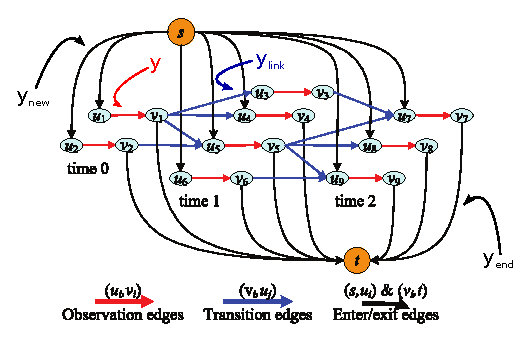
\includegraphics{flow_conv.eps}\\[-1ex]
		{\tiny Credit: Nevatia et al, Global Data Association for Multi-Object Tracking - Edited}}
    {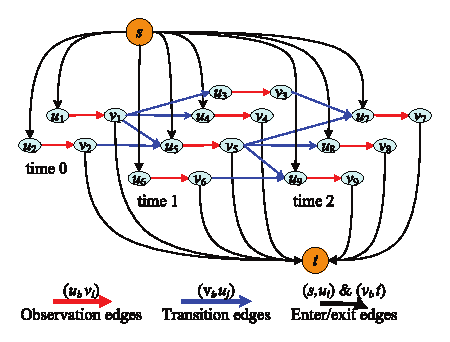
\includegraphics{flow.eps}\\[-1ex]
		{\tiny Credit: Nevatia et al, Global Data Association for Multi-Object Tracking}}
	\end{center}
\end{frame}


%%%%%%%%%%%%%%%%%%%%%%%%%%%%%%%%%%%%%%%%%%%%%%%%%%%%%%
%%%%%%%%%%%%%%%%%%%%%%%%%%%%%%%%%%%%%%%%%%%%%%%%%%%%%%
\begin{frame}{Flow Model}
	\begin{itemize}
		\item This way we can solve our MAP as a Max-Flow problem.
		\begin{itemize}
			\item Each flow path is a trajectory;
			\item Flow conservation guarantees no trajectory overlap;
			\item Amount of flow from \textit{s} to \textit{t} is the number of trajectories.
			\item Total cost of flow is the negative log-likelihood of the trajectories' hipothesis
		\end{itemize}
		\item Global optimality can be guaranteed.
	\end{itemize}
\end{frame}

%%%%%%%%%%%%%%%%%%%%%%%%%%%%%%%%%%%%%%%%%%%%%%%%%%%%%%
%%%%%%%%%%%%%%%%%%%%%%%%%%%%%%%%%%%%%%%%%%%%%%%%%%%%%%
\subsection{Min-Cost Flow}
\begin{frame}{Solving with Min-Cost Flow}
	\begin{algorithm}[H]
		\vspace{5px}
		\KwIn{Observation set $\mathcal{X}$}

		\vspace{10px}
		Build flow graph $\mathcal{G}(\mathcal{X})$\\
		Start with flow 0, $f(\mathcal{G}) = 0$\\
		\While{$f(\mathcal{G}) = 0$ can be augmented}{
			Augment $f(\mathcal{G})$ by 1\\
			Compute current cost with Min-Cost Flow\\
			\If{current cost \textless \ optimal cost}{
				Store current cost as optimal cost
			}
		}
		\Return{global optimum}
	\end{algorithm}
\end{frame}


%%%%%%%%%%%%%%%%%%%%%%%%%%%%%%%%%%%%%%%%%%%%%%%%%%%%%%
%%%%%%%%%%%%%%%%%%%%%%%%%%%%%%%%%%%%%%%%%%%%%%%%%%%%%%
\section{\scshape Linear Program}
\begin{frame}{Linear Program}
	\begin{itemize}
		\item Our formulation can also be interpreted as an Integer Program: We want to find integer assignments to our random variables such that the negative log-likelihood is minimized.
		\item Integer Programming is NP-Hard. However we can relax our problem to a Linear Program.
		\begin{itemize}
			\item Total unimodularity guarantees that we will still find integer solutions.
		\end{itemize}
	\end{itemize}
\end{frame}

%%%%%%%%%%%%%%%%%%%%%%%%%%%%%%%%%%%%%%%%%%%%%%%%%%%%%%
%%%%%%%%%%%%%%%%%%%%%%%%%%%%%%%%%%%%%%%%%%%%%%%%%%%%%%
\subsection{Problem Statement}
\begin{frame}{Linear Program}
	\\[-2ex]
\begin{alignat*}{2}
	\label{eq:linear_problem}
	 \text{Max}&\text{imize: }\\
	 & \sum_{x_j \in \mathcal{X}} \Bigg( y_{new_{x_j}} P(y_{new_{x_j}}) + y_{end_{x_j}} P(y_{end_{x_j}}) + y_j \beta_j + (1-y_j)(1-\beta_j) \Bigg)                                         \\
	 & + \sum_{(x_j,x_k)\in \mathcal{L}}y_{link_{x_j,x_k}}P(y_{link_{x_j,x_k}})\\
	 \text{Sub}&\text{ject To: }\\
	 & y_{new_{x_i}} + \sum_{x_k \in \mathcal{L}(x_i)} y_{link_{x_k,x_i}} = y_{end_{x_i}} + \sum_{x_k \in \mathcal{L}(x_i)} y_{link_{x_i,x_k}} = y_{x_i} \ \ \ \forall x_i \in \mathcal{X}
\end{alignat*}
\begin{itemize}
	\item Where $\mathcal{L}$ denotes the set of detections that can be associated, i.e. are from subsequent frames.
\end{itemize}
\end{frame}


%%%%%%%%%%%%%%%%%%%%%%%%%%%%%%%%%%%%%%%%%%%%%%%%%%%%%%
%%%%%%%%%%%%%%%%%%%%%%%%%%%%%%%%%%%%%%%%%%%%%%%%%%%%%%
\section{\scshape Costs}
\begin{frame}{Finding the Probabilities}
\begin{itemize}
	\item So we have defined ways to solve the association problem, however we still need to find ways to compute the probabilities of our random variables, ie $P(y)$, $P(y_{link})$, $P(y_{new})$, $P(y_{end})$.
	\item In the following we propose some ways to address this.
\end{itemize}
\end{frame}


%%%%%%%%%%%%%%%%%%%%%%%%%%%%%%%%%%%%%%%%%%%%%%%%%%%%%%
%%%%%%%%%%%%%%%%%%%%%%%%%%%%%%%%%%%%%%%%%%%%%%%%%%%%%%
\subsection{Detection Score}
\begin{frame}{Detection Score - $P(y)$}
\begin{itemize}
	\item This score can be either the output of the scorer on the detector or a new network trained to classify true and false positives.
	\item It's important that this score is precise, otherwise you might end up with many fragmentations or false positives.
\end{itemize}
\end{frame}


%%%%%%%%%%%%%%%%%%%%%%%%%%%%%%%%%%%%%%%%%%%%%%%%%%%%%%
%%%%%%%%%%%%%%%%%%%%%%%%%%%%%%%%%%%%%%%%%%%%%%%%%%%%%%
\subsection{Matching Score}
\begin{frame}{Matching Score - $P(y_{link})$}
\begin{itemize}
	\item Many metrics can be used for this, among them we have:
	\begin{itemize}
		\item Bounding box overlap;
		\item Bounding box size;
		\item Color histogram similarity;
		\item Orientation cosine similarity;
		\item Position distance;
		\item ...
	\end{itemize}
	\item As is the case for $y_j$, a poor estimation of this cost may lead to many ID switches.
\end{itemize}
\end{frame}

%%%%%%%%%%%%%%%%%%%%%%%%%%%%%%%%%%%%%%%%%%%%%%%%%%%%%%
%%%%%%%%%%%%%%%%%%%%%%%%%%%%%%%%%%%%%%%%%%%%%%%%%%%%%%
\begin{frame}{Matching Score - $P(y_{link})$}
\begin{center}
	\includegraphics<1>[width=\columnwidth]{f1.jpg}
	\includegraphics<2>[width=\columnwidth]{f2.jpg}
	\includegraphics<3>[width=\columnwidth]{f3.jpg}
\end{center}
\end{frame}


%%%%%%%%%%%%%%%%%%%%%%%%%%%%%%%%%%%%%%%%%%%%%%%%%%%%%%
%%%%%%%%%%%%%%%%%%%%%%%%%%%%%%%%%%%%%%%%%%%%%%%%%%%%%%
\subsection{New/End Scores}
\begin{frame}{New/End Scores - $P(y_{new})$ and $P(y_{end})$}
\begin{itemize}
	\item The costs for $P(y_{new})$ and $P(y_{end})$ are usually constants estimated via the EM Algorithm.
	\item Not particularly important to be set on a per-detection basis.
\end{itemize}
\end{frame}


%%%%%%%%%%%%%%%%%%%%%%%%%%%%%%%%%%%%%%%%%%%%%%%%%%%%%%
%%%%%%%%%%%%%%%%%%%%%%%%%%%%%%%%%%%%%%%%%%%%%%%%%%%%%%
\section{\scshape Metrics}
\begin{frame}{Metrics}
\begin{itemize}
	\item Given a solution to the tracking problem, it's in our interest to have metrics to proper evaluate whether or not the solution satisfies our expectations.
	\item The most widespread metrics for this purpose are the CLEAR MOT and MT/ML metrics.
\end{itemize}
\end{frame}


%%%%%%%%%%%%%%%%%%%%%%%%%%%%%%%%%%%%%%%%%%%%%%%%%%%%%%
%%%%%%%%%%%%%%%%%%%%%%%%%%%%%%%%%%%%%%%%%%%%%%%%%%%%%%
\subsection{CLEAR MOT}
\begin{frame}{MOTA}
\begin{itemize}
	\item \textbf{MOTA} - Multiple Object Tracking Accuracy:
	\begin{itemize}
		\item Accounts for errors in the trajectory configuration: misses, false positives and mismatches.
		\item Gives a measure of how well the tracker is able to detect object and keep consistent trajectories, regardless of the precision with which the object detections are estimated.
	\end{itemize}
	\begin{gather*}
	MOTA = \dfrac{\sum_{t} (m_t, fp_t, mme_t)}{\sum_t g_t}
	\end{gather*}
	\item Where $m_t$, $fp_t$, $mme_t$ and $g_t$ are, respectively, the number of misses, false positives,  mismatches and objects present at time $t$.
\end{itemize}
\end{frame}

%%%%%%%%%%%%%%%%%%%%%%%%%%%%%%%%%%%%%%%%%%%%%%%%%%%%%%
%%%%%%%%%%%%%%%%%%%%%%%%%%%%%%%%%%%%%%%%%%%%%%%%%%%%%%
\begin{frame}{MOTP}
\begin{itemize}
	\item \textbf{MOTP} - Multiple Object Tracking Precision:
	\begin{itemize}
		\item Measures the total error in estimated position between object-hypothesis pairs
		\item Evaluates the tracker's ability of estimating object positions, regardless of its skill of keeping consistent trajectories.
	\end{itemize}
	\begin{gather*}
	MOTP = \dfrac{\sum_{i,t} d_t^i}{\sum_t c_t}
	\end{gather*}
	\item Where $d_t^i$ is the distance between object $o_i$ and its corresponding hypothesis at time $t$ and $c_t$ is the number of matches at time $t$.
\end{itemize}
\end{frame}


%%%%%%%%%%%%%%%%%%%%%%%%%%%%%%%%%%%%%%%%%%%%%%%%%%%%%%
%%%%%%%%%%%%%%%%%%%%%%%%%%%%%%%%%%%%%%%%%%%%%%%%%%%%%%
\subsection{MT/ML}
\begin{frame}{MT/ML}
	\begin{itemize}
		\item \textbf{MT} - Mostly Tracked - evaluates the percentage of trajectories that cover a ground-truth trajectory for more than 80\% of its length.
		\item \textbf{ML} - Mostly Lost - percentage of trajectories that cover a GT trajectory for less than 20\% of its length.
		\item \textbf{PT} - Partially Tracked - $1.0-MT-ML$.
	\end{itemize}
\end{frame}


%%%%%%%%%%%%%%%%%%%%%%%%%%%%%%%%%%%%%%%%%%%%%%%%%%%%%%
%%%%%%%%%%%%%%%%%%%%%%%%%%%%%%%%%%%%%%%%%%%%%%%%%%%%%%
\section{\scshape Online}
\begin{frame}{Online Tracking}
	\begin{itemize}
		\item So far, our optimization scheme follows an offline setting: Given an entire sequence of observations we find the RV assignments with optimal cost.
		\item This approach doesn't scale too well since as the length of the sequence grows, so does the complexity of the LP.
		\item Furthermore, for real time applications (robotics, autonomous driving, broadcasting, etc) we need the tracking output with minimal delay.
	\end{itemize}
\end{frame}


%%%%%%%%%%%%%%%%%%%%%%%%%%%%%%%%%%%%%%%%%%%%%%%%%%%%%%
%%%%%%%%%%%%%%%%%%%%%%%%%%%%%%%%%%%%%%%%%%%%%%%%%%%%%%
\begin{frame}{Online Tracking}
	\begin{itemize}
		\item The min-cost flow approach has a complexity of $O(kn^2m\log n)$, where $k$ is the number of objects, $m$ the number of edges and $n$ the number of nodes in the graph.
		\begin{itemize}
			\item Even if we used a sliding window approach, this complexity would still make the successive re-calculations slow.
		\end{itemize}
		\item Because our tracking graph is a DAG and we want node-disjoint solutions, we can formulate our problem using \textit{k} shortest node-disjoint paths.
		\begin{itemize}
			\item This approach has a complexity of $O(k(m+n\log n))$, making it feasible for online applications.
		\end{itemize}
	\end{itemize}
\end{frame}


%%%%%%%%%%%%%%%%%%%%%%%%%%%%%%%%%%%%%%%%%%%%%%%%%%%%%%
%%%%%%%%%%%%%%%%%%%%%%%%%%%%%%%%%%%%%%%%%%%%%%%%%%%%%%
\begin{frame}{Online Tracking}
	\begin{center}
		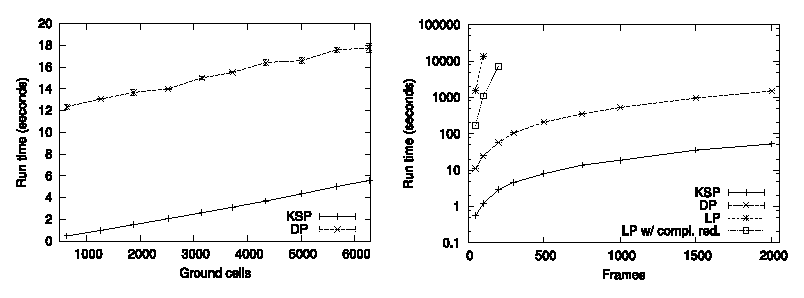
\includegraphics[width=\columnwidth]{ksp_time.eps}\\
		{\tiny Credit: Berclaz et al, Multiple Object Tracking using K-Shortest Paths Optimization}
	\end{center}
\end{frame}


%%%%%%%%%%%%%%%%%%%%%%%%%%%%%%%%%%%%%%%%%%%%%%%%%%%%%%
%%%%%%%%%%%%%%%%%%%%%%%%%%%%%%%%%%%%%%%%%%%%%%%%%%%%%%
\subsection{K-Shortest Node Disjoint Paths}
\begin{frame}{Tracking with KSP}
	\begin{algorithm}[H]
		\vspace{5px}
		\KwIn{Observation set $\mathcal{X}$}

		\vspace{10px}
		Build flow graph $\mathcal{G}(\mathcal{X})$\\
		Start with $k$ = 0\\
		\While{$k$ can be augmented}{
			Augment $k$ by 1\\
			Compute current cost with \textit{KSP}\\
			\If{current cost \textless \ optimal cost}{
				Store current cost as optimal cost
			}
		}
		\Return{global optimum}
	\end{algorithm}
\end{frame}


%%%%%%%%%%%%%%%%%%%%%%%%%%%%%%%%%%%%%%%%%%%%%%%%%%%%%%
%%%%%%%%%%%%%%%%%%%%%%%%%%%%%%%%%%%%%%%%%%%%%%%%%%%%%%
\subsection{Online KSP}
\begin{frame}{Online Tracking with KSP}
	\begin{itemize}
		\item To transform our offline setting into online, we split the sequence into smaller batches that we can efficiently process.
		\item To enforce consistency between batches, we introduce an overlap between each sequence, and make it such that the inward flow of each node is equal to the outward flow in the previous batch.
	\end{itemize}
\end{frame}

%%%%%%%%%%%%%%%%%%%%%%%%%%%%%%%%%%%%%%%%%%%%%%%%%%%%%%
%%%%%%%%%%%%%%%%%%%%%%%%%%%%%%%%%%%%%%%%%%%%%%%%%%%%%%
\begin{frame}{Online Tracking with KSP}
\begin{center}
	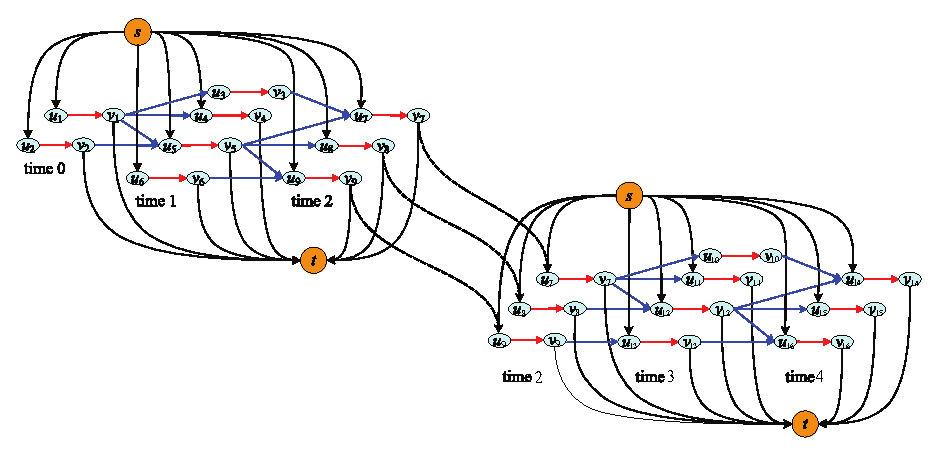
\includegraphics[width=\columnwidth]{online_flow.eps}\\
	{\tiny Credit: Nevatia et al, Global Data Association for Multi-Object Tracking - Edited}
\end{center}
\end{frame}


%%%%%%%%%%%%%%%%%%%%%%%%%%%%%%%%%%%%%%%%%%%%%%%%%%%%%%
%%%%%%%%%%%%%%%%%%%%%%%%%%%%%%%%%%%%%%%%%%%%%%%%%%%%%%
\begin{frame}{Online Tracking with KSP}
	\begin{itemize}
		\item For implementation details and additional information into bounded computation and memory we refer you to:
	\end{itemize}
	\begin{center}
		\url{http://www.cs.toronto.edu/boundTracking/}
	\end{center}
\end{frame}


%%%%%%%%%%%%%%%%%%%%%%%%%%%%%%%%%%%%%%%%%%%%%%%%%%%%%%
%%%%%%%%%%%%%%%%%%%%%%%%%%%%%%%%%%%%%%%%%%%%%%%%%%%%%%
\section{\scshape Continuous}
\begin{frame}{Continuous Optimization}
	\begin{itemize}
		\item So far we've only dealt with discrete assignments, ie we either associate two detections or don't.
		\item This doesn't take into account higher order motion features (speed, acceleration, etc), which will generally produce jagged trajectories.
	\end{itemize}
\end{frame}


%%%%%%%%%%%%%%%%%%%%%%%%%%%%%%%%%%%%%%%%%%%%%%%%%%%%%%
%%%%%%%%%%%%%%%%%%%%%%%%%%%%%%%%%%%%%%%%%%%%%%%%%%%%%%
\begin{frame}{Continuous Optimization}
	\begin{center}
		\movie[autostart,repeat,poster]{\includegraphics[width=\columnwidth]{vid_thumb.png}}{./track.mp4}
	\end{center}
\end{frame}


%%%%%%%%%%%%%%%%%%%%%%%%%%%%%%%%%%%%%%%%%%%%%%%%%%%%%%
%%%%%%%%%%%%%%%%%%%%%%%%%%%%%%%%%%%%%%%%%%%%%%%%%%%%%%
\begin{frame}{Continuous Optimization}
	\begin{itemize}
		\item However, we can do better by using prior knowledge of the domain:
		\begin{itemize}
			\item Cars don't change shape and have predictable motion dynamics according to the road;
			\item The trajectory of a projectile (ball) can be reasonably estimated given speed and acceleration;
			\item People usually move in the direction they are facing.
			\item ...
		\end{itemize}
	\end{itemize}
\end{frame}


%%%%%%%%%%%%%%%%%%%%%%%%%%%%%%%%%%%%%%%%%%%%%%%%%%%%%%
%%%%%%%%%%%%%%%%%%%%%%%%%%%%%%%%%%%%%%%%%%%%%%%%%%%%%%
\begin{frame}{Continuous Optimization}
	\begin{enumerate}
		\item \alt<2>{\textbf{We can encode that information as an additional cost in the objective function and minimize using gradient descent.}}{We can encode that information as an additional cost in the objective function and minimize using gradient descent.} \footnotemark
		\item We can use a filtering technique (Bayes, Kalman, Particle, ...) over each individual trajectory. \footnotemark
		\item We can use Recurrent Neural Networks to estimate smooth trajectories. \footnotemark
	\end{enumerate}
	\footnotetext[1]{\tiny Milan et al., Multi-Target Tracking by Discrete-Continuous Energy Minimization}
	\footnotetext[2]{\tiny Thrun et al., Probabilistic Robotics}
	\footnotetext[3]{\tiny Milan et al., Online Multi-Target Tracking Using Recurrent Neural Networks}
\end{frame}


%%%%%%%%%%%%%%%%%%%%%%%%%%%%%%%%%%%%%%%%%%%%%%%%%%%%%%
%%%%%%%%%%%%%%%%%%%%%%%%%%%%%%%%%%%%%%%%%%%%%%%%%%%%%%
\subsection{Augmented Objective Function}
\begin{frame}{Augmented Objective Function}
	\begin{alignat*}{2}
		\label{eq:linear_problem}
		 O(\mathcal{T}, \mathcal{Y}|\mathcal{X}) = & \sum_{x_j \in \mathcal{X}} \Bigg( y_{new_{x_j}} P(y_{new_{x_j}}|\mathcal{T}) + y_{end_{x_j}} P(y_{end_{x_j}}|\mathcal{T}) + y_{x_j} P(y_{x_j}|\mathcal{T}) \Bigg)                                         \\
		 & + \sum_{(x_j,x_k)\in \mathcal{L}}y_{link_{x_j,x_k}}P(y_{link_{x_j,x_k}}|\mathcal{T})\\
		 & + \mathbf{\sum_{T_j \in \mathcal{T}} P(T_j|\mathcal{Y})}
	 \end{alignat*}
	 \begin{itemize}
	 	\item Notice that we add conditionals to our probabilities since we'll want to use the continuous information in our discrete assignments and vice-versa.
	 \end{itemize}
\end{frame}



%%%%%%%%%%%%%%%%%%%%%%%%%%%%%%%%%%%%%%%%%%%%%%%%%%%%%%
%%%%%%%%%%%%%%%%%%%%%%%%%%%%%%%%%%%%%%%%%%%%%%%%%%%%%%
\begin{frame}{Augmented Objective Function}
\begin{itemize}
	\item With the $P(T_j|\mathcal{Y})$ term we can model higher order functions of our trajectories.
	\begin{itemize}
		\item Impose smooth shapes to trajectories, such as splines;
		\item Constrain their dynamic states to feasible ones;
		\item Filter out noise produced by low scoring detections;
		\item ...
	\end{itemize}
\end{itemize}
\end{frame}



%%%%%%%%%%%%%%%%%%%%%%%%%%%%%%%%%%%%%%%%%%%%%%%%%%%%%%
%%%%%%%%%%%%%%%%%%%%%%%%%%%%%%%%%%%%%%%%%%%%%%%%%%%%%%
\begin{frame}{Augmented Objective Function}
\begin{itemize}
	\item Furthermore, we can exploit motion models to improve our initial trajectory hypothesis
\end{itemize}
\begin{center}
	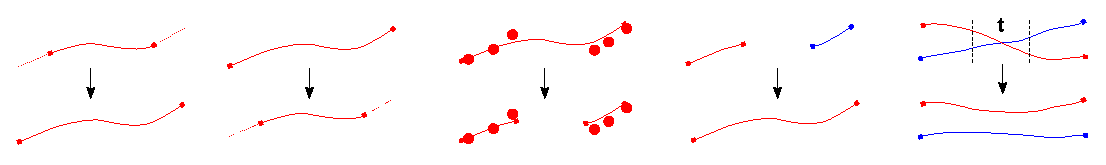
\includegraphics[width=\columnwidth]{fixing.eps}\\[-1ex]
	{\tiny Credit: Milan et al., Multi-Target Tracking by Discrete-Continuous Energy Minimization}
\end{center}
\end{frame}


%%%%%%%%%%%%%%%%%%%%%%%%%%%%%%%%%%%%%%%%%%%%%%%%%%%%%%
%%%%%%%%%%%%%%%%%%%%%%%%%%%%%%%%%%%%%%%%%%%%%%%%%%%%%%
\subsection{Optimization Scheme}
\begin{frame}{Optimization Scheme}
\begin{algorithm}[H]
	\vspace{5px}
	\KwIn{Observation set $\mathcal{X}$}

	\vspace{10px}
	\Repeat{convergence}{
		Minimize $O(\mathcal{T}, \mathcal{Y}|\mathcal{X})$ wrt. $\mathcal{Y}$ via Max-Flow/LP/KSP\\
		Minimize $O(\mathcal{T}, \mathcal{Y}|\mathcal{X})$ wrt. $\mathcal{T}$ via Gradient Descent
	}
	\Return{global optimum}
\end{algorithm}
\end{frame}


%%%%%%%%%%%%%%%%%%%%%%%%%%%%%%%%%%%%%%%%%%%%%%%%%%%%%%
%%%%%%%%%%%%%%%%%%%%%%%%%%%%%%%%%%%%%%%%%%%%%%%%%%%%%%
\section{\scshape Numbers}
\subsection{Matching}
\begin{frame}{Some Numbers - KITTI Dataset}
\begin{itemize}
	\item Matching error rate:
\end{itemize}
\begin{center}
	\begin{table}
	 \begin{tabular}{l|lll}
	   \hline
	   & \multicolumn{3}{c}{\textsc{Error Rate}}\\\hline
	   \textsc{Metric} & \textsc{Mean} & \textsc{Positive} & \textsc{Negative}\\ \hline\hline
	   Cosine Similarity & 29.16\% & 19.02\% & 39.30\%\\
	   Color Correlation & 15.31\% & 20.21\% & 10.41\%\\
	   BBox Size & 6.31\% & 5.27\% & 7.35\%\\
	   BBox Position & 5.13\% & 5.86\% & 4.40\%\\
	   BBox Overlap & 2.46\% & 4.68\% & 0.23\%\\\hline
	   \hline
	 \end{tabular}
	\end{table}
\end{center}
\end{frame}


%%%%%%%%%%%%%%%%%%%%%%%%%%%%%%%%%%%%%%%%%%%%%%%%%%%%%%
%%%%%%%%%%%%%%%%%%%%%%%%%%%%%%%%%%%%%%%%%%%%%%%%%%%%%%
\subsection{Tracking}
\begin{frame}{Some Numbers - KITTI Dataset}
\begin{itemize}
	\item Hungarian X Linear Program:
\end{itemize}
\begin{center}
	\begin{table}
	\resizebox{\textwidth}{!}{
	 \begin{tabular}{llllllll}
	   \hline
	   \textsc{Method} & \textsc{Mota} & \textsc{Motp} & \textsc{Mt} & \textsc{Ml} & \textsc{Ids} & \textsc{Frag} & \textsc{Fp}\\ \hline\hline
	   Hungarian & 58.69\% & 84.26\% & \textbf{70.87\%} & \textbf{6.80\%} & 68 & 196 & 2880 \\\hdashline
	   LP  & \textbf{71.12\%} & \textbf{85.24\%} & 55.66\% & 12.94\% & \textbf{19} & \textbf{99} & \textbf{628}\\
	   \hline
	 \end{tabular}
  }
	\end{table}
\end{center}
\end{frame}


%%%%%%%%%%%%%%%%%%%%%%%%%%%%%%%%%%%%%%%%%%%%%%%%%%%%%%
%%%%%%%%%%%%%%%%%%%%%%%%%%%%%%%%%%%%%%%%%%%%%%%%%%%%%%
\subsection{Detection}
\begin{frame}{Some Numbers - KITTI Dataset}
\begin{itemize}
	\item Real X Ideal detections:
\end{itemize}
\begin{center}
	\begin{table}
	\resizebox{\textwidth}{!}{
	 \begin{tabular}{llllllll}
	   \hline
	   \textsc{Method} & \textsc{Mota} & \textsc{Motp} & \textsc{Mt} & \textsc{Ml} & \textsc{Ids} & \textsc{Frag} & \textsc{Fp}\\ \hline\hline
	   Real & 71.12\% & 85.24\% & 55.66\% & 12.94\% & 19 & 99 & 628 \\\hdashline
	   Ideal & \textbf{79.44\%} & \textbf{89.27\%} & \textbf{72.17\%} & \textbf{6.15\%} & \textbf{7} & \textbf{37} & \textbf{462}\\
	   \hline
	 \end{tabular}
  }
	\end{table}
\end{center}
\end{frame}

\end{document}
